% Attention block mapping figure for §8.1 Tiled attention dataflow.
% Replaces the ASCII score-grid diagram. Color semantics follow the
% FlatAttention paper figures: orange = multicast, magenta = reduce,
% green = local 3D DRAM access.
\documentclass[border=10pt]{standalone}
\usepackage{amsmath,amssymb}
\usepackage{tikz}
\usetikzlibrary{positioning,fit,arrows.meta,calc,backgrounds}

\newcommand{\srcQ}{\mathrm{src}_{Q}}
\newcommand{\srcKV}{\mathrm{src}_{KV}}
\newcommand{\dstO}{\mathrm{dst}_{O}}

\begin{document}
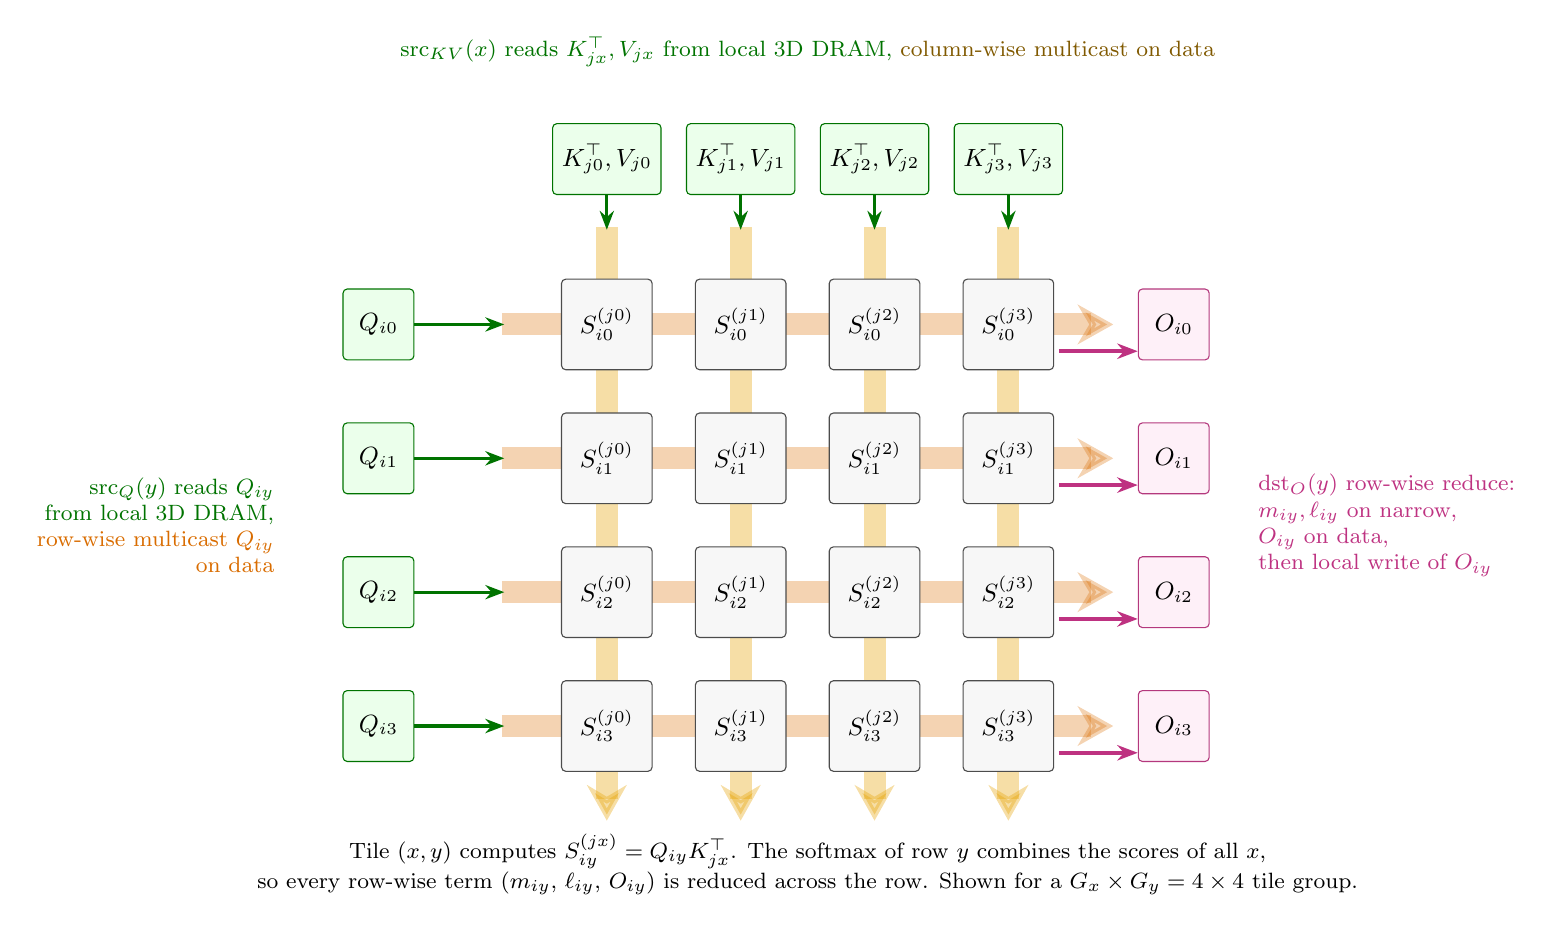
\begin{tikzpicture}[
  cell/.style={draw=black!70, rounded corners=1.5pt, minimum size=11.5mm,
               fill=gray!6, font=\small},
  srcbox/.style={draw=green!45!black, rounded corners=1.5pt, minimum size=9mm,
                 fill=green!8, font=\small, align=center},
  dstbox/.style={draw=magenta!70!black, rounded corners=1.5pt, minimum size=9mm,
                 fill=magenta!6, font=\small, align=center},
  qband/.style={-{Stealth[length=4.5mm, width=5mm]}, line width=2.8mm,
                orange!85!black, opacity=0.30},
  kband/.style={-{Stealth[length=4.5mm, width=5mm]}, line width=2.8mm,
                orange!60!yellow!90!black, opacity=0.35},
  red/.style={-{Stealth[length=2.6mm]}, line width=1.3pt, magenta!75!black},
  feed/.style={-{Stealth[length=2.4mm]}, line width=1.2pt, green!45!black},
  note/.style={font=\footnotesize, align=left},
]

% ---- score grid: cell (x,y), x rightward, y downward ----
\foreach \x in {0,1,2,3}
  \foreach \y in {0,1,2,3}
    \node[cell] (c\x\y) at (1.7*\x, -1.7*\y) {$S_{i\y}^{(j\x)}$};

% ---- Q sources, one per row (left) ----
\foreach \y in {0,1,2,3} {
  \node[srcbox] (q\y) at (-2.9, -1.7*\y) {$Q_{i\y}$};
  \draw[feed] (q\y.east) -- ($(c0\y.west)-(0.72,0)$);
}

% ---- K/V sources, one per column (top) ----
\foreach \x in {0,1,2,3} {
  \node[srcbox] (kv\x) at (1.7*\x, 2.1) {$K^{\top}_{j\x}, V_{j\x}$};
  \draw[feed] (kv\x.south) -- ($(c\x0.north)+(0,0.62)$);
}

% ---- multicast bands behind the cells ----
\begin{scope}[on background layer]
  \foreach \y in {0,1,2,3}
    \draw[qband] ($(c0\y.west)-(0.75,0)$) -- ($(c3\y.east)+(0.75,0)$);
  \foreach \x in {0,1,2,3}
    \draw[kband] ($(c\x0.north)+(0,0.65)$) -- ($(c\x3.south)-(0,0.62)$);
\end{scope}

% ---- O owners, one per row (right) ----
\foreach \y in {0,1,2,3} {
  \node[dstbox] (o\y) at (7.2, -1.7*\y) {$O_{i\y}$};
  \draw[red] ($(c3\y.east)+(0.06,-0.34)$) -- ($(o\y.west)+(0,-0.34)$);
}

% ---- side notes ----
\node[note, green!45!black, anchor=east, align=right] at (-4.1, -2.55)
  {$\srcQ(y)$ reads $Q_{iy}$\\from local 3D DRAM,\\
   \textcolor{orange!85!black}{row-wise multicast $Q_{iy}$}\\
   \textcolor{orange!85!black}{on data}};

\node[note, green!45!black, anchor=south, align=center] at (2.55, 3.15)
  {$\srcKV(x)$ reads $K^{\top}_{jx}, V_{jx}$ from local 3D DRAM,
   \textcolor{orange!60!yellow!50!black}{column-wise multicast on data}};

\node[note, magenta!75!black, anchor=west, align=left] at (8.15, -2.55)
  {$\dstO(y)$ row-wise reduce:\\
   $m_{iy}, \ell_{iy}$ on narrow,\\
   $O_{iy}$ on data,\\
   then local write of $O_{iy}$};

% ---- caption line under the grid ----
\node[note, anchor=north, align=center] at (2.55, -6.35)
  {Tile $(x,y)$ computes $S_{iy}^{(jx)} = Q_{iy} K^{\top}_{jx}$.
   The softmax of row $y$ combines the scores of all $x$,\\
   so every row-wise term ($m_{iy}$, $\ell_{iy}$, $O_{iy}$) is reduced across the row.
   Shown for a $G_x \times G_y = 4 \times 4$ tile group.};

\end{tikzpicture}
\end{document}
